\documentclass[../main.tex]{subfiles}

\begin{document}
\section{Consumatori}

I \textbf{consumatori} sono agenti economici disposti a pagare per acquistare beni o servizi.

Così come le imprese mirano a massimizzare il profitto, i \textbf{consumatori acquistano beni o servizi per aumentare il proprio benessere (utilità)}

\subsection{Utilità}

\textbf{Utilità}: misura della soddisfazione che si ricava dal consumo di beni e servizi.

La \textbf{funzione di utilità} descrive come varia il livello di soddisfazione del consumatore al variare delle quantità di beni e servizi consumati. Tipicamente valgono le seguenti condizioni:
\begin{itemize}
\item \textbf{Utilità monotona e crescente}: il consumo di un determinato bene fa aumetare l'utilità al consumatore.
\item \textbf{Utilità marginale decrescente}: l'utilità addizionale (marginale) di ogni successiva unità di consumo è via via minore. Esempio: la prima birra la bevo molto volentieri, la seconda la gradisco comunque ma leggermente meno, alla decima non la gradisco proprio.
\end{itemize}

\subsection{Prezzo di riserva}

\textbf{Prezzo di riserva (PR)}: prezzo massimo che un consumatore è disposto a pagare per acquistare un'unità di un bene.

Il prezzo di riserva guida le decisioni di acquisto:
\begin{itemize}
\item PR $>$ Prezzo praticato da imprese produttrici $\rightarrow$ Acquisto
\item PR $<$ Prezzo praticato da imprese produttrici $\rightarrow$ Non acquisto
\end{itemize}

Conoscere il prezzo di riserva consente di costruire la curva di domanda individuale.

\subsection{Curva di domanda individuale}

\textbf{Curva di domanda individuale di un bene x}: esprime, per ciascun consumatore, il prezzo di riserva di diverse quantità di x.

La curva di domanda individuale è \textbf{decrescente}. Se il prezzo sale, la quantità domandata dal consumatore scende, e viceversa.

Il prezzo di riserva è legato all'utilità marginale:
\begin{itemize}
\item  il prezzo di riserva dipende dalla quantità di bene già consumata.
\item la variazione di utilità in seguito al consumo di un'unità aggiuntiva del bene (unità marginale) è decrescente.
\end{itemize}

La curva di domanda individuale consente di valutare il \textbf{surplus del consumatore}: differenza fra il prezzo che un consumatore è disposto a pagare e il prezzo di mercato del bene. Esempio: se sono disposto a pagare 5 euro per una birra, e la vendono a 3 euro, il surplus è 2 euro.\\

\subsubsection{Determinanti della domanda individuale:}
\begin{enumerate}
\item Caratteristiche del consumatore
	\begin{itemize}
	\item \textbf{Gusti e necessità}
	\item \textbf{Reddito o ricchezza}: questo può influenzare la domanda in due modi diversi a seconda del tipo di bene:
		\begin{itemize}
		\item Beni normali: la quantità domandata aumenta all'aumentare del reddito.
		\item Beni inferiori: la quantità domandata diminuisce all'aumentare del reddito.
		\end{itemize}
	\end{itemize}
\item Caratteristiche del bene
	\begin{itemize}
	\item \textbf{Prezzo e disponibilità di beni sostituti}, ovvero beni che espletano funzioni simili a quelle di x. Se aumenta (diminuisce) il prezzo di un sostituto di x, la quantità domandata di x aumenta (diminuisce).
	\item \textbf{Prezzo e disponibilità di beni complementari}, ovvero beni che tendono ad essere consumati insieme ad x. Se aumenta (diminuisce) il prezzo di un bene complementare a x, la quantità domandata di x diminuisce (aumenta).
	\end{itemize}
\end{enumerate}

\subsection{Domanda di mercato}

\textbf{Domanda di mercato} (domanda aggregata): somma, per tutti gli N consumatori, delle quantità domandate individuali
$$Q(p) = \sum_{i=1}^N\,q_i(p)$$

La domanda di mercato può avere varie forme funzionali, ma è comunque (quasi) sempre descrescente.

\subsubsection{Elasticità della domanda}

L'elasticità della domanda è la variazione percentuale della quantità domandata al variare di una delle sue componenti: prezzo del bene, prezzo degli altri beni e reddito del consumatore.

Una misurazione accurata della variazione della domanda consente di conoscere le reazioni dei consumatori e quindi l'impatto che tali variazioni hanno sui ricavi dell'impresa.\\

\textbf{Elasticità della domanda al prezzo} del bene x: variazione percentuale della quantità domandata del bene x a seguito della variazione percentuale del suo prezzo.
$$
\varepsilon_x=\frac{\frac{\Delta q_x}{q_x}}{\frac{\Delta p_x}{p_x}}\Rightarrow\varepsilon_x=\frac{\Delta q_x}{\Delta p_x}\frac{p_x}{q_x}\Rightarrow\varepsilon_x=\frac{\partial q_x}{\partial p_x}\frac{p_x}{q_x}
$$

è in genere negativa, si considera solo il valore assoluto
$$
\varepsilon_x = |\frac{\partial q_x}{\partial p_x}\frac{p_x}{q_x}|
$$

Esempio di bene caratterizzato da bassa elasticità della domanda al prezzo: acqua (in generale tutti i beni di prima necessità).

\begin{itemize}
\item La domanda di un bene con \textbf{pochi sostituti} è \textbf{poco elastica (anelastica)}
\item La domanda di un bene con \textbf{molti sostituti} è \textbf{molto elastica (elastica)}\\
\end{itemize}

\textbf{Elasticità incrociata} del bene x rispetto a y: variazione percentuale della quantità domandata di x rispetto ad una variazione percentuale del prezzo del bene y
$$\varepsilon_{xy}=\frac{\partial q_x}{\partial p_y}\frac{p_y}{q_x}$$
Il segno dipende dalle relazioni di complementarietà e sostituibilità tra i beni
\begin{itemize}
\item \textbf{Beni complementari}: elasticità incrociata \textbf{negativa}.
\item \textbf{Beni sostituti}: elasticità incrociata \textbf{positiva}.\\
\end{itemize}

\textbf{Elasticità della domanda al reddito} del bene x: variazione percentuale della quantità domandata del bene x a seguito della variazione percentuale del reddit M
$$\varepsilon_M=\frac{\partial q_x}{\partial M} \frac{M}{q_x}$$

\begin{itemize}
\item \textbf{Beni normali}: elasticità della domanda al reddito \textbf{positiva}.
\item \textbf{Beni inferiori}: elasticità della domanda al reddito \textbf{negativa}.
\end{itemize}

\section{Offerta e forme di mercato}

Una decisione fondamentale per le imprese è definire la \textbf{quantità q di un bene da produrre per massimizzare il profitto} $\pi$, definito come:
$$\pi(q) = RT(q) - CT(q)$$
Per trovare il massimo in funzione della quantità q, si calcola la derivata prima e si uguaglia a 0:
$$\max_q \pi = \frac{\partial \pi(q)}{\partial q}=RM(q) - CM(q) = 0$$
$$\mathbf{RM(q) = CM(q)}$$
\begin{itemize}
\item $\mathbf{RM(q)}$ \textbf{ricavo marginale}: derivata prima del ricavo, rappresenta il ricavo ottenuto servendo un cliente aggiuntivo.
\item $\mathbf{CM(q)}$ \textbf{costo marginale}: derivata prima del cost, rappresenta il corso di servire un cliente aggiuntivo.
\end{itemize}

L'impresa considera di servire un cliente in più solo se effettivamente servire quel cliente aggiuntivo genera profitti addizionali, e non rappresenta un costo marginale maggiore del ricavo marginale.

La capacità delle imprese di massimizzare il profitto dipende da \textbf{fattori di mercato} quali
\begin{itemize}
    \item \textbf{Numero di concorrenti} (imprese che producono beni che i consumatori percepiscono come stretti sostituti).
    \item \textbf{Natura del prodotto} (omogeneo vs. differenziato).
    \item \textbf{Grado di libertà di entrata} (o uscita) delle imprese nel mercato.
    \item \textbf{Quantità dell'informazione} detenuta da imprese e consumatori.
    \item \dots
\end{itemize}

Tali caratteristiche definiscono la \textbf{forma di mercato (livello di competizione)} in cui opera l'impresa.

I mercati si collocano in un continuum tra concorrenza perfetta e monopolio
\begin{itemize}
    \item \textbf{Concorrenza perfetta}: infinite imprese nell'azienda, massimo livello di competizione.
    \item \textbf{Monopolio}: una sola impresa nell'industria, minimo livello di competizione.
\end{itemize}

\subsection{Concorrenza perfetta}

Il modello di concorrenza perfetta si basa su \textbf{quattro ipotesi fondamentali}.
\begin{enumerate}
    \item Esiste un \textbf{numero molto elevato di imprese} nel mercato; la singola impresa produce una quota trascurabile dell'offerta totale.
    \item Tutte le imprese producono un \textbf{prodotto identico}; in altre parole, il prodotto è omogeneo (non differenziato).
    \item Acquirenti e venditori hanno una \textbf{conoscenza perfetta} dei prodotti e dei prezzi.
    \item Esiste \textbf{completa libertà di entrata e di uscita} da parte di nuove imprese.
\end{enumerate}

Non esiste un mercato che soddisfa perfettamente le condizioni elencate sopra, ma ci sono esempi che si avvicinano: \emph{mercato ortofrutticolo}, molti produttori, i prodotti venduti sono tutti gli stessi. Queste attività non sono particolarmente lucrative, fare profitti elevati è difficile.

La concorrenza perfetta è una \textbf{forma di mercato estrema}:
\begin{itemize}
    \item Le imprese non hanno alcun potere di influenzare il prezzo del prodotto.
    \item Il prezzo a cui vendono è determinato dall'interazione della domanda e dell'offerta complessiva di mercato (si veda dopo).
\end{itemize}

In altri termini le \textbf{imprese sono price-taker}
\begin{itemize}
    \item Se fissassero un \textbf{prezzo superiore} a quello di mercato, \textbf{non venderebbero nulla}.
    \item Se fissassero un \textbf{prezzo inferiore} a quello di mercato, \textbf{non avrebbero la capacità di soddisfare l'intero mercato}. Gli altri produttori continuano a vendere al loro prezzo e fanno più soldi, quindi non conviene.
\end{itemize}

\textbf{Qual è la quantità q che consente all'impresa di massimizzare il profitto (= ricavi - costi)?}

\subsubsection{Curva di offerta individuale}
La curva di offerta individuale esprime, \textbf{per ogni livello di prezzo p, la quantità ottimale q di produzione del bene}.

\begin{figure}[h]
    \centering
    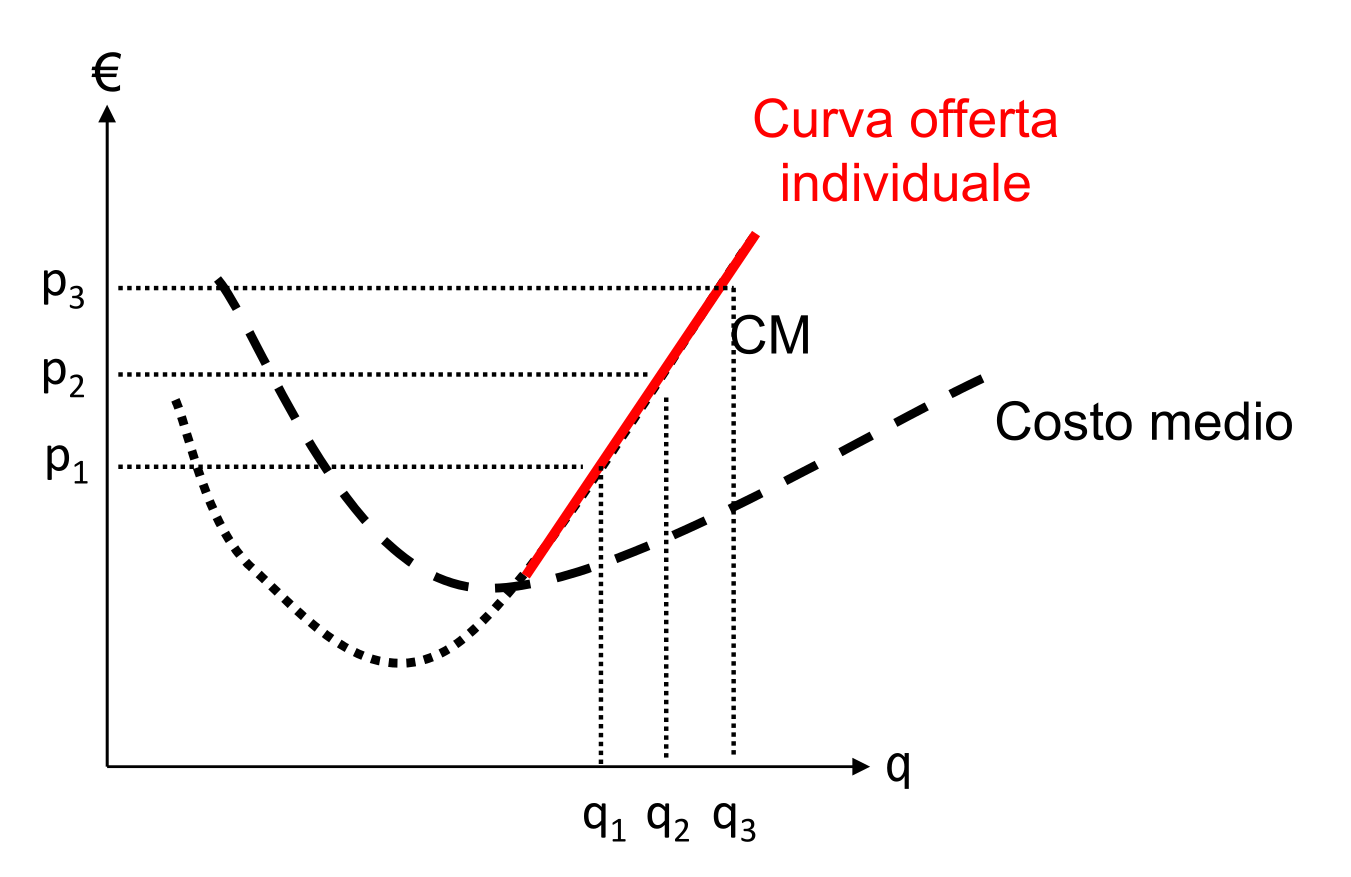
\includegraphics[width=0.8\textwidth]{curva-offerta-individuale.png}
\end{figure}

Essendo l'impresa price-taker, p non dipende dalla quantità prodotta dalla singola impresa q:
$$RT(q) = p\cdot q$$
$$RM(q) = p$$

\textbf{Condizione di massimizzazione del profitto}: $RM(q) = CM(q)$. Si ottiene quindi:
$$p = CM(q)$$

\textbf{Condizione minima di produzione}: $\pi = pq - CT(q) > 0$.

Si ottiene quindi che il prezzo deve essere superiore al costo medio affinchè l'impresa sia in grado di ottenere profitti positivi.
$$\mathbf{p > \frac{CT(q)}{q}}$$

\subsubsection{Curva di offerta di mercato}
La curva di offerta di mercato è la somma delle curve di offerta di tutte le imprese nel mercato.

\begin{figure}[h]
    \centering
    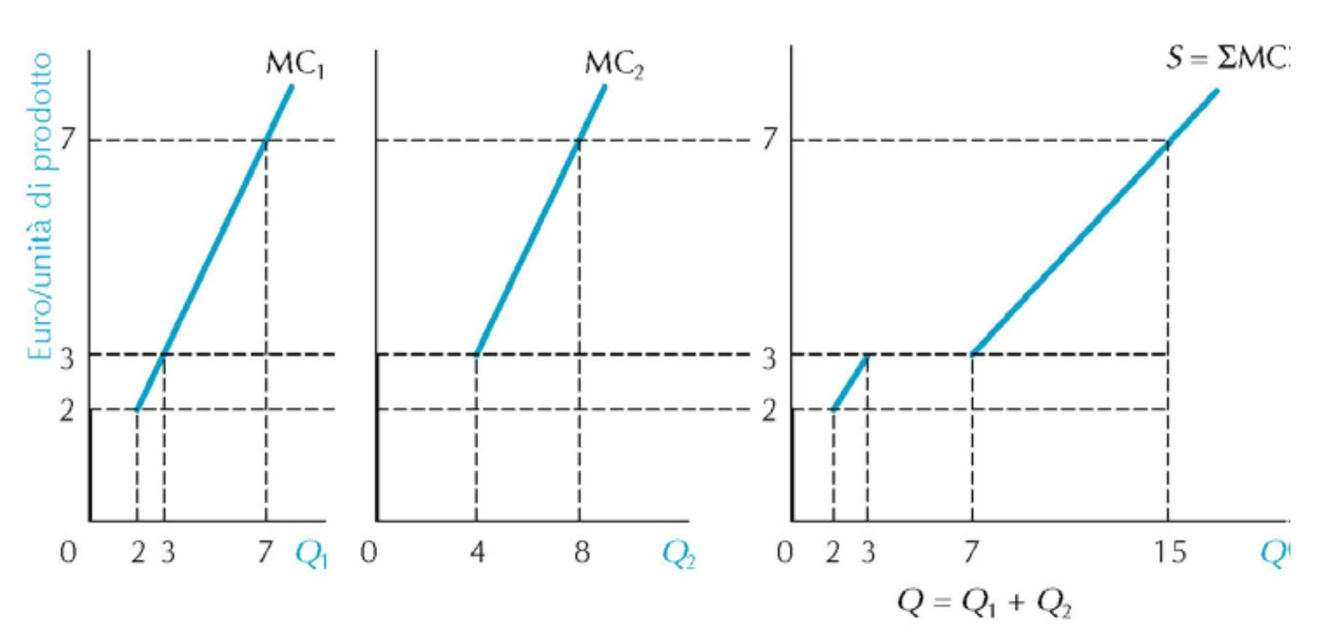
\includegraphics[width=0.95\textwidth]{curva-offerta-mercato.png}
\end{figure}

Se in un mercato in cui operano molteplici aziende produttrici, il \textbf{prezzo di equilibrio} dipende dall'\textbf{incontro tra domanda e offerta di mercato}.

\begin{itemize}
    \item \textbf{Se p $>$ prezzo di equilibrio di mercato} si verifica un \textbf{eccesso di offerta}, ovvero alcuni produttori non riescono a vendere. Di conseguenza il prezzo si abbassa per vendere di più, anche ai consumatori con prezzo di riserva più basso.
    \item \textbf{Se p $<$ prezzo di equilibrio di mercato} si verifica un \textbf{eccesso di domanda}, ovvero alcuni consumatori sarebbero disposti a comprare il bene ma questo non sarebbe disponibile.
\end{itemize}

Nel lungo periodo, se le imprese già operative ottengono profitti positivi (p $>$ costo medio), \textbf{nuove imprese saranno attirate nel mercato}.

La dinamica del prezzo nel mercato ha quindi un \textbf{andamento ciclico}:

\begin{itemize}
    \item nuove imprese entrano nel mercato attratte dal profitto.
    \item l'offerta sale e il prezzo di equilibrio scende.
    \item per alcune imprese diviene p $<$ costo medio.
    \item le imprese con costo medio $>$ p escono dal mercato.
    \item l'offerta scende e il prezzo sale
    \item \dots e così via.
\end{itemize}

\textbf{Equilibrio di lungo periodo}: entrata e uscita cessano quando non sono più possibili profitti. Rimangono sul mercato solo le imprese più efficienti che producono al costo medio minimo. Le \textbf{imprese conseguono profitti nulli}.

\textbf{Dal punto di vista dell'impresa, la concorrenza non è desiderabile.}

\subsection{Monopolio}

A volte in un mercato c'è un'\textbf{unica impresa produttrice} (monopolista). 
Questo si verifica nel caso in cui esistono ostacoli insormontabili (le barriere all'entrata) che impediscono ad altre imprese di entrare e competere.

Il monopolista è \textbf{price-maker}:
\begin{itemize}
    \item A differenza della concorrenza perfetta, \textbf{fronteggia l'intera curva di domanda di mercato}.
    \item \textbf{Il prezzo al quale egli vende il prodotto non è indipendente dalla quantità venduta.}
\end{itemize}

Ne consegue che i ricavi totali sono dati da:
$$RT(q) = p(q)\cdot q$$
Ed il ricavo marginale è quindi:
$$
RM(q)=\frac{\partial p(q)}{\partial q}\cdot q + p(q) = p(q)\cdot \left(\frac{\partial p(q)}{\partial q}\frac{q}{p(q)}+1\right)=p(q)\cdot \left(-\frac{1}{\varepsilon}+1\right)
$$
Dove $\varepsilon$ è l'elasticità della domanda al prezzo (in valore assoluto).

Si applica la \textbf{condizione di massimizzazione del profitto}: $RM(q) = CM(q)$, e si ottiene quindi
$$p(q)\cdot \left(-\frac{1}{\varepsilon}+1\right)=CM(q)$$
$$\mathbf{\frac{p(q)-CM(q)}{p(q)} = \frac{1}{\bm\varepsilon}}$$

Il monopolista fissa un prezzo al di sopra dei costi marginali (si dice che ha \textbf{potere di mercato}). Il potere di mercato è tanto maggiore quanto meno la domanda risponde alle variazioni di prezzo.

\end{document}